El almacenamiento de votos es importante a corto y largo plazo. Es necesario poder obtener un resultado correcto al momento de finalizar la elección, pero también deben estar disponibles los datos si se quisiera hacer un recuento en el futuro. 
Por lo visto, no hay una única forma de almacenar los votos durante el sufragio y se utilizan diversas formas para tal. Desde distintos medios de almacenamiento como tarjetas RIFT hasta la propia memoria de la maquina de votación, donde no necesariamente es excluyente alguna de las dos.  
Mencionaremos distintas técnicas que se utilizaron en distintos países, y los agujeros de seguridad que se encontraron en tales.

\subsection{Estados Unidos}
En este país encontramos un caso que nos llama la atención ya que se utiliza criptografía en el voto electrónico pero no es utilizada correctamente. Como dice el paper 
\footnote{\url{http://www.engr.uconn.edu/~sad06005/pubs/Conference/sac12.pdf}}
que leímos sobre tal votación,la mera utilización de herramientas criptográficas puede conducir a una falsa sensacion de seguridad. Con el fin de ser eficaz, la criptografía debe ser utilizado en conjunción con un buen diseño que proporcione una protección completa en la integridad de la información crítica.

En el paper mencionado, cuenta que para emitir votos de forma electrónica se utilizó la terminal de votación AccuVote TSX, utilizada por más de 12 millones de votantes en más de 350 jurisdicciones en los EE.UU.  Los votos son almacenados en una tarjeta PCMCIA.

Esta terminal tiene vulnerabilidades en la integridad de la información que permite un ataque que intercambia los votos de dos candidatos y otro que borra el nombre de un candidato. Ambos ataques son capaces de eludir las comprobaciones de integridad de cifrado implementados en la terminal. Los ataques se pueden iniciar en cuestión de minutos y sólo requieren una computadora con la capacidad para montar una tarjeta PCMCIA. No es necesario que el atacante tenga información de la elección que va a fraudentar, solo es necesario que tenga acceso a la maquina de votación para abrir el compartimiento donde se almacena la tarjeta PCMCIA.

Las vulnerabilidades encontradas en el paper fueron:
\begin{itemize}
	\item Aunque el nombre de cada candidato está acompañado por 128 bits de integridad, la terminal no los usa de forma efectiva. Cuando falla el chequeo de integridad en un candidato, no se cuenta el voto para este candidato. Aunque el elector verifique en la boleta VVPAT que figura el candidato de forma correcta, su voto no será tenido en cuenta para el recuento de votos ya que el recuento electrónico lo realiza con lo almacenado en la tarjeta PCMCIA y al fallar la integridad del candidato, no lo cuenta. Tampoco existe una verificación de la integridad de que no se cambió los nombres de candidatos en los recuentos de los votos
	\item Tampoco hay una firma criptográfica de la tarjeta PCMCIA. Por ende, se puede agregar más contenido a la urna de votación
	\item La existencia de puertas traseras como en versiones anteriores de la terminal y un mecanismo de actualización de archivos débil ya que tan solo se utiliza el nombre del archivo a actualizar para identificar una actualización de software válida
	\item Las máquinas de votación tienen la misma llave física para obtener la tarjeta PCMCIA, al menos en las que fueron revisadas
\end{itemize}

Otra falla relacionada al almacenamiento que existió en estados unidos durante una elección 
\footnote{\url{http://usatoday30.usatoday.com/news/politicselections/vote2004/2004-11-04-votes-lost_x.htm}}
 utilizando el voto electrónico fue que más de 4.500 votos se perdieron en un condado de Carolina del Norte, porque las autoridades creían una maquina de votación electrónica podrían contener más datos de lo que efectivamente almacenaba.

\subsection{India}
Este país nos resultó interesante ya que es el país democrático más grande. En elecciones nacionales recientes, más votos fueron contados que juntando la población de Estados Unidos con Canadá, y la mayoría de los electores, votaron utilizando el voto electrónico.
El componente electronico de votacion en India, llamado EVM, está compuesto por dos partes: la unidad de votación (izquierda) y la unidad de control (derecha) que están enlazadas por un cable de 5 metros. Las unidades de votación están realizadas para soportar hasta 16 candidatos. En caso de ser más candidatos, se agrega otra unidad de votacion y es posible agregar hasta 4 unidades de votación, dando una capacidad máxima de 64 posibles candidatos.   En la unidad de votación, se agrega una hoja indicando que boton representa a cada candidato con el simbolo de su partido politico. Para votar, el elector tiene que ser identificado por el presidente de mesa que luego le realiza una marca en el dedo con tinta indeleble para evitar que vuelva a votar y presiona un botón en la unidad de control, permitiendo al elector votar en la unidad de votacion. Al realizar esto, se prende una luz en la unidad de votación indicando que el votante está listo para sufragar.

\begin{figure}[h]
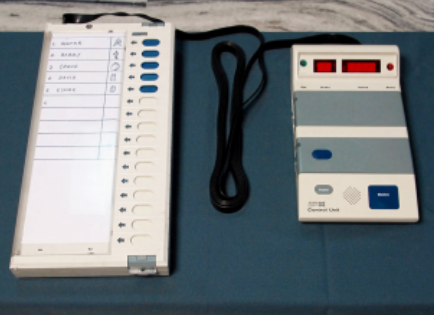
\includegraphics{Imagenes/almacenamiento1}
\caption{Maquina de votacion electronica utilizada en India }
\end{figure}

Las vulnerabilidad encontrada en el paper leído es
\footnote{\url{https://jhalderm.com/pub/papers/evm-ccs10.pdf}}
que se puede reemplazar fácilmente algún componente del equipo sea CPU, placas o agregar hardware. Los diseñadores de las EVM podían haber hecho los ataques más difíciles agregando un mecanismo criptográfico para identificar a los distintos componentes de hardware originales, como un mecanismo de challengeResponde basado en un secreto contenido en el firmware original. 
Un posibles ataques mencionados en el paper es Dishonest Display.
Se desarrolló una placa de visualización que puede reemplazar a la placa real en la unidad de control. Normalmente cuando los votos son contados, la cantidad de votos recibidos por cada candidato figura en el tablero real. Con el ataque, el tablero agrega un microcontrolador que intercepta los votos totales y realiza la sustitución fraudulenta de resultados emitiendose en el tablero de visualización. Notar que en este ataque hay que realizar un intercambio de un componente de hardware.

\begin{figure}[h]
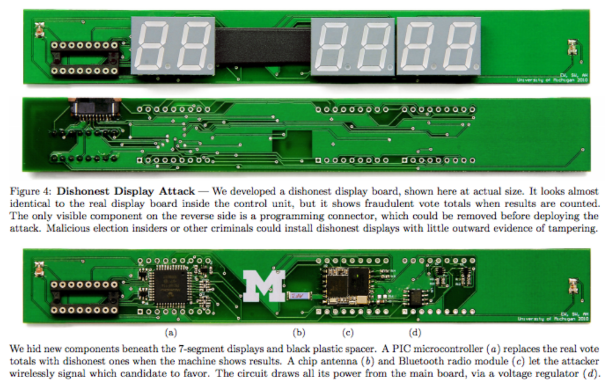
\includegraphics[width=0.8\textwidth]{Imagenes/almacenamiento2}
\caption{Hardware utilizado}
\end{figure}

Además, el paper menciona otra ataque más pero optamos comentarlo en la sección de privacidad ya que tiene más relación con la pérdida del anonimato.
Un detalle no menor, es que el recuento de votos de la  elección en India se realiza semanas después del sufragio. Por ende, el atacante tiene tiempo para poder realizar el cambio o agregar hardware que le permite realizar el ataque mientras están almacenadas.

\subsection{Holanda}
Este país
\footnote{\url{https://www.ndi.org/e-voting-guide/netherlands-CS/opposition-to-e-voting}}  
\footnote{\url{http://wijvertrouwenstemcomputersniet.nl/English}}  
 nos llamó la atención porque debido la fuerza mediática que tuvo en la sociedad la difusión de un video
\footnote{\url{http://www.veoh.com/watch/v505707dgewqMsB}}  
 sobre las máquinas de votación NEDAP podían ser manipuladas,  se logró volver a votar en papel y lápiz, como se votaba anteriormente en este país.  
Sucedió algo similar al caso de India: se necesitaban 5 minutos para poder manipular una de estas máquinas NEDAP cambiando dos chips, y como estas estaban guardadas sin una seguridad correspondiente al tema en cuestión, cualquier persona podia modificarlas.

\subsection{Argentina e Israel}
Otra forma de almacenar los votos, es la implementada en las elecciones del 2015 en Argentina y en las elecciones previas al 2010 en Israel, donde los votos se grababan en un chip RFID que se encontraba en la boleta (En el caso de Argentina sería la BUE) y se deposita la boleta en una urna física. Luego, en el escrutinio de votos, se utiliza una maquina para leer la información de la boleta y poder contabilizar el voto. En la sección de privacidad, seguiremos mencionando estos países ya que los comentarios acerca de los posibles ataques tienen más que ver con la pérdida del anonimato que con el formato de almacenamiento en si.